\section{Diskussion}
\label{sec:Diskussion}

Die rote Linie der Cd-Lampe entsteht durch den Übergang
$^1\mathrm{P}_1 \leftrightarrow\, ^1\mathrm{D}_2$,
welcher in Abbildung \ref{fig:termschema-rot} dargestellt ist.
Da beide Zustände einen Gesamtspin $S = \num{0}$ haben, ist hier
der normale Zeeman-Effekt zu beobachten und eine Aufspaltung der
$\pi$-Linie ist nicht zu erwarten.
Des Weiteren ist ein $\zeta$ von \num{1} zu erwarten.
\begin{figure}
	\centering
	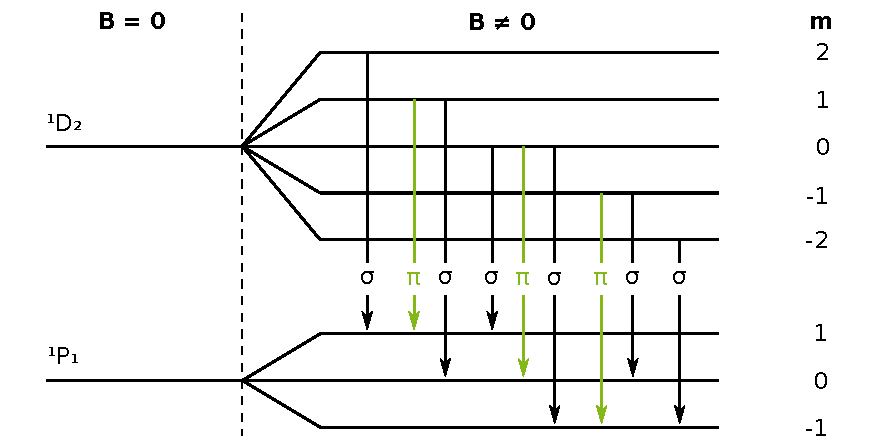
\includegraphics{images/termschema-rot.pdf}
	\caption{Termschema für die rote Linie der \ce{Cd}-Lampe.}
	\label{fig:termschema-rot}
\end{figure}

Die blaue Linie der Cd-Lampe entsteht durch den Übergang
$^3\mathrm{P}_1 \leftrightarrow\, ^3\mathrm{S}_1$,
welcher in Abbildung \ref{fig:termschema-blau} dargestellt
ist. Hier wird der anormale Zeeman-Effekt beobachtet.
Für die $\pi$-Übergänge gilt $\zeta = \num{0.5}$, während
für die $\sigma$-Übergänge \num{1.5} und \num{2} gilt.
Diese beiden Linien können in diesem Experiment jedoch nicht
unabhängig voneinander untersucht werden, sodass hier der
Mittelwert \num{1.75} als Theoriewert erwartet wird.
\begin{figure}
  \centering
  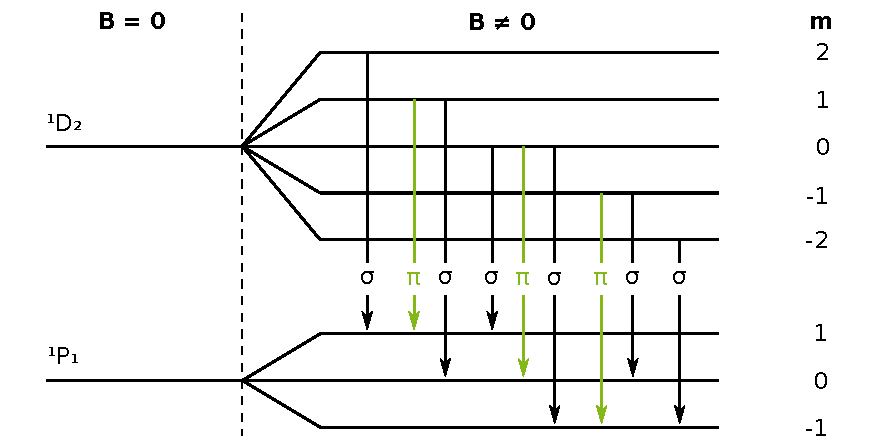
\includegraphics{images/termschema-blau.pdf}
  \caption{Termschema für die blaue Linie der \ce{Cd}-Lampe.}
  \label{fig:termschema-blau}
\end{figure}

\begin{table}
  \centering
  \caption{Vergleich der experimentell bestimmten Werte von $\zeta$ mit den
  theoretisch berechneten.}
  \label{tab:ergebnisse}
  \begin{tabular}{
    c
    S[table-format=1.2]
    S[table-format=1.2] @{${}\pm{}$} S[table-format=1.2]
    }
  \toprule
    {Spektrallinie} &
    {Theorie} &
    \multicolumn{2}{c}{Messung} \\
  \midrule
    $\sigma$ Rot & 1 & 0.96 & 0.10 \\
    $\sigma$ Blau & 1.75 & 1.95 & 0.12 \\
    $\pi$ Blau & 0.5 & 0.48 & 0.13 \\
  \bottomrule
  \end{tabular}
\end{table}
In Tabelle \ref{tab:ergebnisse} sind die gemessenen und theoretisch berechneten
Werte für $\zeta = \left|\Delta\left(m g\right)\right|$ dargestellt.
Es zeigt sich, dass bis auf den $\sigma$-Übergang der blauen Linie die experimentell
bestimmten Werte im Rahmen ihrer Unsicherheit mit den theoretisch berechneten
Werten übereinstimmen. Diese Abweichung, jedoch auch die generelle Unsicherheit der
experimentell bestimmten Werte zwischen \num{0.1} und \num{0.13} lassen sich auf eine Reihe von möglichen
Ursachen zurück führen.

Zum einen können systematische Fehler durch eine ungenaue Eichung entstanden sein.
Die verwendete Hallsonde konnte nicht befestigt werden, sodass sie während der gesamten
Messung mit der Hand festgehalten wurde und eine Reproduzierbarkeit der Daten nicht
gewährleistet ist. Weiterhin ließ sich die Lampe nicht aus der Halterung entfernen,
sodass die Sonde nicht exakt das Feld an der Cd-Lampenposition vermessen hat.
Dies kann zu großen Abweichungen geführt haben, da das magnetische Feld nur
begrenzt homogen war.
% - Bei Stromstärken ~19A kurzschluss, sodass effektiv nur Felder bis ~18A nutzbar.

Das Prisma der Lummer-Gehrcke-Platte hatte weiterhin eine Bruchstelle, sodass
ungewollte Reflexe innerhalb des Prismas und damit auch innerhalb der Platte
entstanden sein können. Diese Reflexe reduzieren dann die Intensität des
ausfallenden Interferenzlichts.
Der größte Faktor ist jedoch die manuelle Justage der einzelnen optischen
Komponenten. Bei unpräziser Justage verringert sich die Intensität des
von der Kamera aufgenommenen Lichts erheblich. Dies wird die Hauptursache sein,
warum die Bilder der roten Linie deutlich dunkler sind als die Bilder der
blauen Spektrallinie.

Um die Auswertung der roten Linie möglichst präzise durch zu führen, wurde anstelle
des Bildes ohne angelegtes externes Magnetfeld das Bild des $\pi$-Lichtes bei
\SI{0.64(7)}{\tesla} eingelesen. Die Übereinstimmung im Rahmen der Unsicherheit mit
dem theoretischen Wert zeigt jedoch, dass diese Methode so anwendbar ist.

Schließlich hängt die Güte der bestimmten Werte von $\zeta$ erheblich davon ab, wie
genau die Maxima der einzelnen horizontalen Schnitte durch die Bilder bestimmt werden
konnten. Hier lagen die zu bestimmenden Maxima bei eingeschaltetem Magnetfeld
meist sehr nahe aneinander, sodass die Bestimmung der Maxima nicht eindeutig ist.
Aus diesem Grund konnten auch nicht alle mit dem Auge sichtbaren Maxima in die
Auswertung eingebunden werden. Besonders bei der Auswertung der roten
Spektrallinie ist dieser Effekt aufgrund der geringen Intensität der Maxima
ausgeprägt.
